\id{IRSTI 28.23.29}{https://doi.org/10.58805/kazutb.v.4.25-400}

\begin{articleheader}
\sectionwithauthors{N.B Assymkhan, A.Z.Kartbaev}{THERMAL COMFORT PREDICTION USING SVM AND RANDOM FOREST MODEL}

{\bfseries N.B. Assymkhan\textsuperscript{\envelope }, A. Kartbaev}
\end{articleheader}

\begin{affiliation}
Kazakh-British Technical University, Almaty, Kazakhstan

\raggedright {\bfseries \textsuperscript{\envelope }}Correspondent-author anb.asymhan@gmail.com
\end{affiliation}

Predicting thermal comfort is crucial for optimizing built environments
for human habitation, as it impacts health, productivity, and overall
well-being. To address this imperative, interdisciplinary colla\-boration
among architects, engineers, psychologists, and data scientists is
needed to develop reliable predic-tive models that anticipate occupants'
thermal comfort preferences across diverse environmental conditions and
architectural designs. Traditional methods rely on human comfort models,
which can be subjective and time-consuming. Machine learning algorithms,
such as Support Vector Machines (SVM) and Random Forest (RF), have been
utilized to predict thermal comfort with high accuracy and efficiency.
The Internet of Things (IoT) is revolutionizing the building management
systems industry, with adaptive control \\algorithms and modular
architectures exploring the IoT paradigm. This paper discusses the use
of SVM and Random Forest algorithms for predicting thermal comfort in
buildings, exploring their strengths and weaknesses and comparing their
performance in different scenarios. The study analyzed a dataset of
thermal comfort data, filtering by quantity and removing outliers. The
data was split into 80\% for training and 20\% for testing. The study
used SVM and Random Forest models to capture complex relationships
between environmental parameters and thermal comfort responses. The
results showed that the IQR method provided 3-4\% accuracy, while the
reducing label values method offered 20-23\% accuracy. The study also
tested the parameters of the models, resulting in a 2-4\% difference
between the two models. The study concluded that Random Forest appears
more stable than SVM and plans to add new features to improve accuracy.

{\bfseries Keywords:} Heating, ventilation, and air conditioning,
temperature, thermal comfort, support vector machine (SVM), random
forest (RF).

\begin{articleheader}
{\bfseries ПРОГНОЗИРОВАНИЕ ТЕПЛОВОГО КОМФОРТА С ПОМОЩЬЮ МОДЕЛИ SVM И RANDOM
FOREST}
\end{articleheader}

\begin{affiliation}
{\bfseries Н.Б.Асымхан\textsuperscript{\envelope }, А. Картбаев}

Казахстанско-Британский Технический Университет,Алматы, Казахстан,

e-mail: anb.asymhan@gmail.com
\end{affiliation}

Прогнозирование теплового комфорта имеет решающее значение для
оптимизации строительных сред для человеческого проживания, так как оно
влияет на здоровье, производительность и общее благополучие. Для решения
этой задачи требуется междисциплинарное сотрудничество архитекторов,
инженеров, психологов и специалистов по обработке данных для разработки
надежных прогностических моделей, предвидящих предпочтения жильцов к
тепловому комфорту в различных климатических условиях и архитектурных
решениях. Традиционные методы основаны на моделях комфорта человека,
которые могут быть субъективными и затратными по времени. Алгоритмы
машинного обучения, такие как Support Vector Machine (SVM) и Random
Forest (RF), использовались для прогнозирования теплового комфорта с
высокой точностью и эффективностью. Интернет вещей (IoT)
революционизирует отрасль систем управления зданиями, с адаптивными
управляющими алгоритмами и модульными архитектурами, исследующими
парадигму IoT. В данной статье обсуждается использование алгоритмов SVM
и Random Forest для прогнозирования теплового комфорта в зданиях,
исследуются их преимущества и недостатки, а также сравнивается их
производительность в различных сценариях. В рамках исследования был
проанализирован набор данных по тепловому комфорту, произведена
фильтрация по количеству и удаление выбросов. Данные были разделены на
80\% для обучения и 20\% для тестирования. В исследовании использовались
модели SVM и Random Forest для выявления сложных взаимосвязей между
параметрами окружающей среды и реакциями на тепловой комфорт. Результаты
показали, что метод IQR обеспечил точность в 3-4\%, в то время как метод
уменьшения значений меток предоставил точность в 20-23\%. Также были
проверены параметры моделей, что привело к различию в 2-4\% между двумя
моделями. Исследование заключает, что Random Forest оказался более
устойчивым, чем SVM, и планирует добавить новые функции для повышения
точности.

{\bfseries Ключевые слова:} отопление, вентиляция и кондиционирование
воздуха, температура, тепловой комфорт, Support Vector Machine (SVM),
Random Forest (RF).

\begin{articleheader}
{\bfseries SVM ЖӘНЕ RANDOM FOREST МОДЕЛДЕРІН ПАЙДАЛАНУ АРҚЫЛЫ ЖЫЛУЛЫҚ ЖАЙЛЫЛЫҚТЫ БОЛЖАУ}

{\bfseries Н.Б. Асымхан\textsuperscript{\envelope }, А. Картбаев}
\end{articleheader}

\begin{affiliation}
Қазақстан-Британ Техникалық Университеті, Алматы, Қазақстан,

e-mail: anb.asymhan@gmail.com
\end{affiliation}

Жылулық жайлылықты болжау адам тұруы үшін салынған ортаны оңтайландыру
үшін өте маңызды, өйткені ол денсаулыққа, өнімділікке және жалпы
әл-ауқатқа әсер етеді. Бұл мәселені шешу сәулетшілер, инженерлер,
психологтар және деректер ғалымдары арасындағы әртүрлі климаттық және
сәулеттік дизайндағы тұрғынның жылулық жайлылық қалауларын болжайтын
сенімді болжамды модельдерді әзірлеу үшін пәнаралық ынтымақтастықты
талап етеді. Дәстүрлі әдістер субъективті және уақытты қажет ететін адам
жайлылық үлгілеріне сүйенеді. Support Vector Machine (SVM) және Random
Forest (RF) сияқты машиналық оқыту алгоритмдері жоғары дәлдік пен
тиімділікпен термиялық жайлылықты болжау үшін пайдаланылды. Заттардың
интернеті (IoT) парадигмасын зерттейтін адаптивті басқару алгоритмдері
мен модульдік архитектуралары арқылы ғимараттарды басқару жүйелерінің
индустриясында төңкеріс жасайды. Бұл мақалада ғимараттардағы жылулық
жайлылықты болжау үшін SVM және Random Forest алгоритмдерін пайдалану
талқыланады, олардың артықшылықтары мен кемшіліктері зерттеледі және
әртүрлі сценарийлердегі олардың өнімділігі салыстырылады. Зерттеудің бір
бөлігі ретінде термиялық жайлылық деректерінің жиынтығы талданды, саны
бойынша сүзілді және шектен тыс мәндер жойылды. Деректер оқу үшін 80\%
және тестілеу үшін 20\% бөлінді. Зерттеу қоршаған орта параметрлері мен
жылулық жайлылық реакциялары арасындағы күрделі қатынастарды анықтау
үшін SVM және Random Forest үлгілерін пайдаланды. Нәтижелер
көрсеткендей, IQR әдісі 3-4\% дәлдік береді, ал жапсырманы азайту әдісі
20-23\% дәлдік береді. Модельдердің параметрлері де тексерілді,
нәтижесінде екі модель арасында 2-4\% айырмашылық болды. Зерттеу Random
Forest SVM-ге қарағанда сенімдірек екенін дәлелдеді және дәлдікті
жақсарту үшін жаңа мүмкіндіктерді қосуды жоспарлап отырмыз.

{\bfseries Tүйін сөздер:} жылыту, желдету және ауаны баптау, температура,
термиялық жайлылық, Support Vector Machine (SVM), Random Forest (RF).

\begin{multicols}{2}
{\bfseries Introduction.} In the pursuit of optimizing built environments
for human habitation, predicting thermal comfort emerges as a pivotal
challenge. With climate change intensifying, the frequency and severity
of extreme weather events are increasing, amplifying the significance of
understanding and managing indoor thermal conditions. The need to
predict thermal comfort stems from its profound impact on human health,
productivity, and overall well-being. Inadequate thermal conditions,
whether excessive heat or cold, can lead to discomfort, fatigue, and
even health complications, thereby compromising individuals' quality of
life and impeding productivity in various settings, including
workplaces, educational institutions, and residential spaces.

Furthermore, the economic implications of disregarding thermal comfort
cannot be overlooked. Suboptimal indoor climates contribute to increased
energy consumption as occupants resort to heating or cooling systems to
mitigate discomfort, resulting in inflated utility bills and
environmental repercussions. Hence, there is a pressing need to develop
reliable predictive models that anticipate occupants' thermal comfort
preferences across diverse environmental conditions and architectural
designs. These models should consider factors such as ambient
temperature, humidity levels, clothing insulation, metabolic rates, and
individual preferences to furnish accurate assessments of thermal
comfort levels. Addressing this imperative requires interdisciplinary
collaboration among architects, engineers, psychologists, and data
scientists to integrate knowledge from environmental science, human
physiology, and behavioral psychology. By leveraging advancements in
sensor technology, data analytics, and machine learning algorithms,
predictive models can be refined to offer real-time insights into
thermal comfort dynamics, empowering building managers and occupants to
optimize indoor environments for enhanced well-being and sustainable
resource utilization. Let's look at how this all affects in more detail
and with an example. Many people know that temperature is a very
important factor for a person, when you start to get sick, the
temperature of your blood rises and this gives you a signal that you
have been poisoned or caught a cold. In a word, it signals that
something has gone wrong in your body. Now how does the room temperature
affect and why do we need a comfortable temperature? For example,
consider a summer day when you start preparing for lessons or studying
something, you close the door of your room so that the noise does not
interfere with your studies and close the window because it is hot
outside. But, here the opposite effect occurs, since you closed the
door, you reduced the area of the room and the speed of airflow into
your room. Further, carbon dioxide will be released, which will fill the
room, thereby reducing the oxygen in the room and increasing the
temperature of the room. Thus, you become a little distracted and
lethargic. You can correct the situation by opening the door of the
room. Also, when you are late for a lesson or a meeting or an exam, you
will release a stress hormone that will increase your body temperature
and your heart rate, given that not only you are sitting in the exam,
but about 40 people and everyone has an increased level of stress and
this affects the fact that oxygen is quickly absorbed and replaced by
carbon dioxide. This will heat up the temperature of the classrooms and
reduce the efficiency level of the students inside. And therefore,
usually at the beginning of the exam, some questions are not clear, then
as the stress level decreases, then clarity of mind opens up. Usually,
the door is opened for this because it has become hot, but there are
HVAC or NV systems for this, which sometimes turn off or they do not
work correctly. Thus, if the comfortable temperature recognition system
works correctly, then by choosing the temperature, you can reduce the
level of stress that will be at the beginning of the exam, thereby
increasing efficiency. If it's cold in the classrooms, usually people
fall asleep, you can notice it when you arrive early at 8 in the morning
for the first lessons, this is because the human body feels cold and
goes into an energy-saving mode like bears in hibernation. That's why
thermal comfort prediction is a crucial aspect of building design and
management as it determines the satisfaction level of occupants in a
given space. Predicting thermal comfort involves analyzing various
factors such as temperature, humidity, air velocity, and clothing
insulation. Traditional methods of predicting thermal comfort rely on
human comfort models, which can be subjective and time-consuming. In
recent years, machine learning algorithms, such as Support Vector
Machines (SVM) and Random Forest (RF), have been utilized to predict
thermal comfort with high accuracy and efficiency. SVM and RF are both
supervised learning algorithms that can be trained on a dataset of
thermal comfort parameters and their corresponding human feedback to
accurately predict thermal comfort in new environments.

{\bfseries Literature review.}The Internet of Things (IoT) is
revolutionizing the building management systems industry, with the
number of connected devices expected to reach 125 billion by 2030.
However, the current BMS solutions are limited in flexibility,
particularly in feedback control options. To fully harness the IoT
paradigm, adaptive control algorithms and modular architectures have
been explored.

The authors propose the ''Semantically-Enhanced IoT-enabled Intelligent
Control System'' (SEMIoTICS) architecture, which exploits redundancy in
control system capabilities and automatically implements alternative
configurations based on quality-of-service criteria {[}1{]}. A study
introduces a novel model that excludes gender and age factors in thermal
comfort assessment. The model considers six thermal factors: air
temperature, mean radiant temperature, relative humidity, air speed,
clothing insulation, and metabolic rate. The model is designed using
Supervised Machine Learning in a commercial building {[}2{]}. A study in
Bilbao, Spain, analyzes human thermal perception in response to external
temperatures using KUBIK, an energy efficiency research facility, to
improve indoor comfort and reduce energy consumption {[}3{]}. This study
evaluates indoor thermal comfort using Fanger method and ASHRAE Standard
55, focusing on real-world conditions to maintain well-being,
productivity, and energy conservation in buildings {[}4{]}. This study
introduces a multiple preferencesbased model for predicting group
thermal comfort in shared spaces, integrating individual preferences and
environmental parameters. It segments occupants based on BMI, predicts
individual comfort zones, and adjusts for group satisfaction {[}5{]}.
Thermal comfort optimization in buildings is crucial for occupant
well-being, productivity, and energy efficiency. Assessment involves
models considering air temperature, humidity, radiant temperature, and
speed. ASHRAE 55 standards define acceptable conditions. Alternative
models like Artificial Neural Networks, hybrid ANN-fuzzy models, SVM,
decision trees, fuzzy logic, and Bayes networks offer flexibility and
accuracy {[}6{]}. Thermal comfort is a crucial aspect of indoor
environmental quality, categorized into static, adaptive, and
data-driven models. Static models like PMV, which integrate
environmental and personal factors, have limitations. Adaptive models
consider psychological and behavioral factors, while data-driven models
use sensor technology for realtime assessments {[}7{]}. The authors
develop a building thermal model using low-resolution data from smart
thermostats, enhancing accuracy and applicability across seasons. They
adapt traditional empirical models into a data-driven approach, using
surrogate features to approximate heat gains. The model can be
implemented on edge devices or cloud infrastructure, offering advantages
in data collection, model learning, and deployment {[}8{]}. Research on
indoor thermal comfort has focused on innovative cooling systems like
Thermoelectric Air Duct. Neural network models have shown accuracy in
predicting comfort parameters, especially in dynamic environments. The
relationship between climatic variables, occupant comfort, and system
performance is crucial {[}9{]}. Thermal comfort prediction and energy
optimization in buildings are crucial for occupant satisfaction and
energy efficiency. Factors influencing comfort include metabolic rate,
clothing insulation, and air temperature. Deep feedforward neural
networks and reinforcement learning models help predict comfort levels.
Monitoring and optimizing HVAC energy consumption is essential for
building operation {[}10{]}. The authors present a novel methodology
using machine learning, data mining, and statistics to develop
predictive models for Combined Heat, Cooling, and Power (CHCP) systems.
The methodology includes four stages: data preparation, data
engineering, model building, and model evaluation. Data preparation
involves retrieving failure events, labeling instances, and creating a
comprehensive dataset. Data engineering enhances data representation
through feature extraction and feature selection. The model building
uses machine learning algorithms for classification and regression
tasks. Model evaluation considers time to failure (TTF) and performance
metrics for suitable selection {[}11{]}. The study explores thermal
comfort in indoor environments using a novel approach called Relative
Thermal Sensation (RTS). The RTS considers thermal sensation as a
continuous function of time, providing a more nuanced understanding of
human thermal sensation. The authors propose a 3-point RTSS to gather
real-time data on relative thermal sensation, capturing subtle changes
in thermal perception that traditional discrete scales may not capture.
The study also integrates RTS data with Absolute Thermal Sensation data
from modified versions of the ASHRAE 7-point thermal sensation scale to
develop a more comprehensive understanding of thermal comfort {[}12{]}.
Interpretable thermal comfort systems are being explored to improve
energy efficiency and occupant satisfaction in smart building
environments. Traditional models like the Predicted Mean Vote (PMV) are
often uninterpretable, making it difficult for building operators to
understand the underlying mechanisms driving thermal comfort.
Researchers have proposed interpretable thermal comfort systems using
machine learning techniques like Partial Dependence Plots (PDP) and SHAP
values. These techniques help operators understand the impact of
environmental conditions on human comfort and the importance of
different features under varying conditions. Additionally, interpretable
ML algorithms can be used to develop surrogate models of existing
comfort models {[}13{]}.

In this paper, we will discuss the use of SVM and Random Forest
algorithms for predicting thermal comfort in buildings. We will explore
their strengths and weaknesses and compare their performance in
different scenarios. The aim of this study is to provide a comprehensive
understanding of the potential of these machine learning algorithms in
predicting thermal comfort, which can help to build designers and
facility managers optimize the indoor environment and improve the
comfort of building occupants.

{\bfseries Materials and Methods.} The primary objective of this study is
to offer a comprehensive understanding of the potential of machine
learning algorithms in predicting thermal comfort. This knowledge can be
instrumental in assisting designers and facility managers in optimizing
the indoor environment, ultimately enhancing the comfort of building
occupants.

\emph{Hypotheses:}

Before commencing our experiments, we have formulated the following
hypotheses:

1) Data Preprocessing:

- It is essential to remove NaN values and set boundaries on the number
of values in each column to ensure the selection of appropriate
features.

- Utilizing the IQR (Interquartile Range) method for label value
reduction to handle outliers effectively.

2) Encoder Selection:

- The choice of encoder, whether it be OneHotEncoder, LabelEncoder, or
Word2Vec, will be critical in transforming categorical variables into a
format suitable for machine learning algorithms.

3) Feature Selection with SelectKBest:

- Utilizing the SelectKBest model will assist us in identifying a list
of features that are most relevant to the thermal comfort prediction.

4) Feature Filtering:

- After initial filtering, we will choose variants of the features that
closely correlate with temperature predictions.
\end{multicols}

\begin{figure}[H]
	\centering
	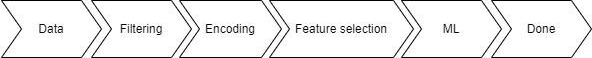
\includegraphics[width=0.6\textwidth]{media/ict/image17}
	\caption*{Figure 1 -- Steps}
\end{figure}

\begin{multicols}{2}
\begin{enumerate}
\def\labelenumi{\Alph{enumi}.}
\item
  \emph{Dataset}
\end{enumerate}

The data was taken from the Kaggle dataset which was taken from the
ASHRAE dataset {[}14{]}. The data has 70 columns and 107583 rows.

\begin{enumerate}
\def\labelenumi{\Alph{enumi}.}
\setcounter{enumi}{1}
\item
  \emph{Filtering data}
\end{enumerate}

In the beginning, after looking at the description of the data, we do
filtering, when viewing it, it turned out that some columns have little
data. Because of this, filtering by quantity went on, and 60.000 lines
were taken by the border. Below this boundary, all data was deleted,
then it was necessary to remove the Nan value, some rows could remain
empty because we had 107583 rows from the beginning. One more hypothesis
to test, the idea is to use \emph{IQR} (Inter Quartile Range) method to
remove outliers if it is exist.
\end{multicols}

\begin{figure}[H]
	\centering
	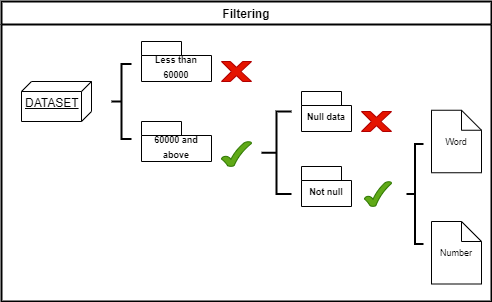
\includegraphics[width=0.8\textwidth]{media/ict/image18}
	\caption*{Figure 2 - Filtering scheme}
\end{figure}

\begin{enumerate}
\def\labelenumi{\Alph{enumi}.}
\setcounter{enumi}{2}
\item
  \emph{Encoding}
\end{enumerate}

\begin{figure}[H]
	\centering
	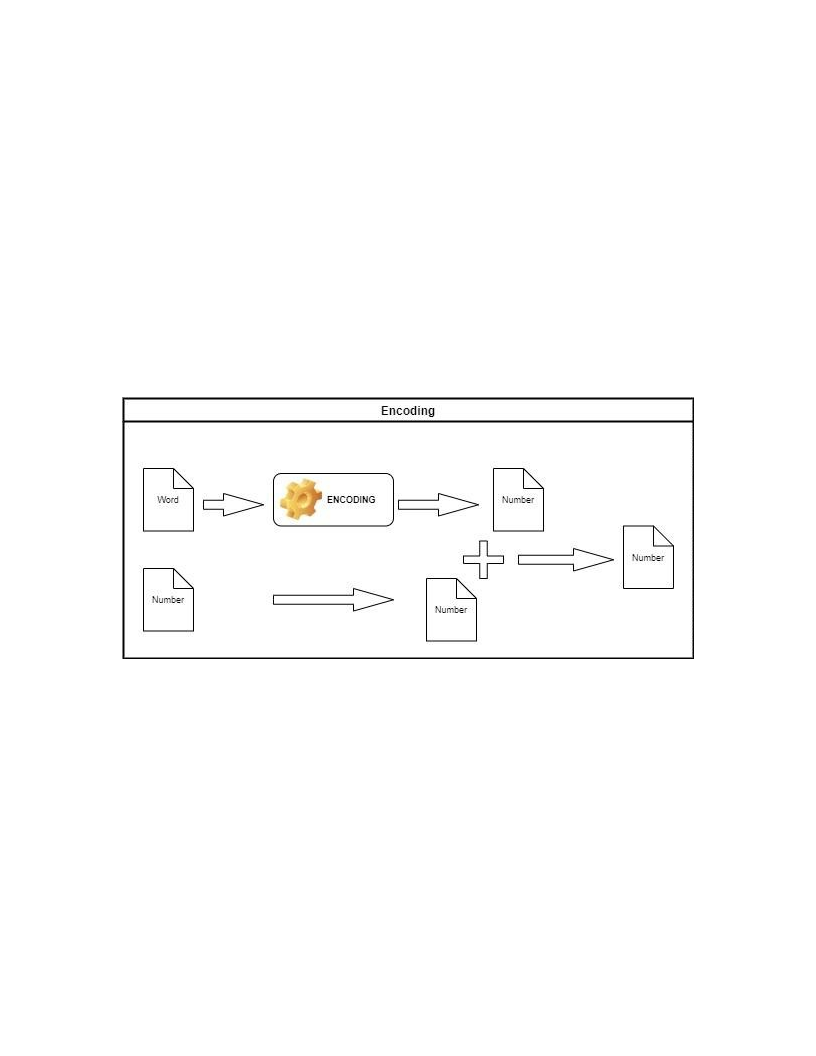
\includegraphics[width=0.8\textwidth]{media/ict/image19}
	\caption*{Figure 3 - Encoding scheme}
\end{figure}

\begin{multicols}{2}
When converting text to a number, there were two choices LabelEncoder or
OneHotEncoder, the choice stopped at One- HotEncoder as it showed good
results.

\begin{enumerate}
\def\labelenumi{\Alph{enumi}.}
\setcounter{enumi}{3}
\item
  \emph{Feature selection}
\end{enumerate}

When choosing a feature, there were two ways to select using the
SelectBest library or a correlation with some kind of restriction and
with the hypothesis. The choice settled on correlations using a boundary
above 50\% of correlations. For features, was used (Age, Clo, Sex, Met,
Thermal preference, Year, Season, Koppen climate classification, Cooling
strat- egy building level, City, PPD, Air temperature (C), Outdoor
monthly air temperature (C), Relative humidity (\%), Air velocity (m/s))
columns. This showed features are the final result, before that we
tested a lot of feature combinations. All combinations and variations
will be presented in the Experi- ment section. As you can see, new
features were added that helped improve the accuracy. The dataset was
split into 80\% for training and 20\% for testing. Thermal comfort
columns usually contained

values from 1 to 6. The next hypothesis, convert label values to
integers. We will have unique 6 values, from 6 unique digits, we reduce
thermal comfort values to 3 digits, which significantly improves
accuracy.
\end{multicols}

\begin{figure}[H]
	\centering
	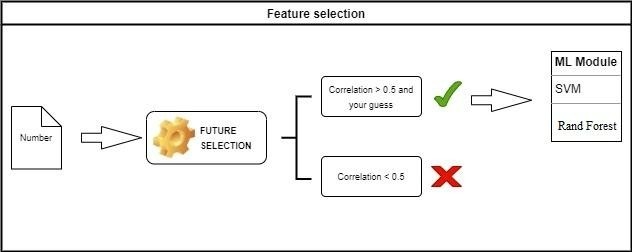
\includegraphics[width=0.8\textwidth]{media/ict/image20}
	\caption*{Figure 4 - Feature selection}
\end{figure}

\begin{multicols}{2}
\begin{enumerate}
\def\labelenumi{\Alph{enumi}.}
\setcounter{enumi}{4}
\item
  \emph{Inter Quartile Range (IQR)}
\end{enumerate}

The Interquartile Range (\emph{IQR}) is a statistical measure that
represents the spread or dispersion of a dataset. The Interquartile
Range (\emph{IQR}) is a measure of statistical dispersion that is
calculated as the difference between the third quartile (\emph{Q}3) and
the first quartile (\emph{Q}1) of a dataset. Mathematically, it is
defined as:

\emph{IQR} = \emph{Q}3 \emph{− Q}1

where \emph{Q}1 is the median of the lower half of the dataset and
\emph{Q}3 is the median of the upper half of the dataset.

The Interquartile Range (\emph{IQR}) is a statistical measure used to
assess the spread or dispersion of a dataset. It is particularly useful
in identifying and dealing with outliers, which are data points that
significantly differ from the rest of the dataset.

Here's how the \emph{IQR} is calculated and how it can be used to remove
outliers:

\emph{Calculation of IQR}:

\begin{itemize}[leftmargin=*]
\item
  Firstly, you need to arrange your dataset in ascend- ing order.
\item
  Then, find the median of the dataset, which is the middle value when
  the data is sorted. If the dataset has an odd number of observations,
  the median is the middle value. If it has an even number of
  observations, the median is the average of the two middle values.
\item
  Divide the dataset into two halves at the median. The lower half
  contains all the values less than or equal to the median, and the
  upper half contains all the values greater than or equal to the
  median.
\item
  Find the median of each half. This gives you the first quartile
  (\emph{Q}1) and the third quartile (\emph{Q}3) of the dataset,
  respectively.
\item
  The Interquartile Range (\emph{IQR}) is then calculated as the
  difference between \emph{Q}3 and \emph{Q}1: \emph{IQR} = \emph{Q}3
  \emph{- Q}1.
\end{itemize}

\emph{Identifying outliers using IQR}:

\begin{itemize}[leftmargin=*]
\item
  Outliers can be detected using the \emph{IQR} method by considering
  values that lie below \emph{Q}1 \emph{−} 1\emph{.}5 \emph{×}
  \emph{IQR} or above \emph{Q}3 + 1\emph{.}5 \emph{× IQR}. These values
  are considered to be significantly different from the rest of the
  dataset.
\item
  Values below \emph{Q}1 \emph{−} 1\emph{.}5 \emph{× IQR} or above
  \emph{Q}3 + 1\emph{.}5 \emph{×} \emph{IQR} are commonly referred to as
  lower and upper bounds, respectively.
\item
  Any data points falling outside these bounds can be considered
  outliers.
\end{itemize}

\emph{Removing outliers using IQR}:

\begin{itemize}[leftmargin=*]
\item
  Once outliers are identified using the \emph{IQR} method, you can
  choose to remove them from the dataset to improve the robustness of
  your analysis or model.
\item
  Outliers can be removed by filtering the dataset to exclude any
  observations that fall outside the lower and upper bounds defined by
  \emph{Q}1 \emph{−} 1\emph{.}5 \emph{× IQR} and
\end{itemize}

\emph{Q}3 + 1\emph{.}5 \emph{× IQR}, respectively.

\begin{itemize}[leftmargin=*]
\item
  After removing outliers, the dataset may be more representative of the
  underlying distribution and less influenced by extreme values.
\end{itemize}

\emph{Considerations}:

\begin{itemize}[leftmargin=*]
\item
  While the \emph{IQR} method is effective in identifying and removing
  outliers, it's important to exercise caution and consider the context
  of the data.
\item
  Outliers may sometimes carry valuable informa- tion or be indicative
  of rare but important events. Therefore, the decision to remove
  outliers should be made judiciously based on the specific goals of the
  analysis or model.
\item
  Additionally, the choice of the multiplier (1.5 in the conventional
  method) used to define the bounds can be adjusted depending on the
  desired level of sensitivity to outliers.
\end{itemize}

In summary, the Interquartile Range (\emph{IQR}) is a useful statistical
measure for assessing the spread of a dataset and identifying outliers.
By calculating the \emph{IQR} and defining bounds based on it, outliers
can be effectively detected and removed, leading to a more robust
analysis or model.

\begin{enumerate}[leftmargin=*]
\def\labelenumi{\Alph{enumi}.}
\setcounter{enumi}{5}
\item
  \emph{Support Vector Machine (SVM)}
\end{enumerate}

Support Vector Machine is a powerful supervised machine learning
algorithm used for classification and regression tasks. SVM works by
finding the optimal hyperplane that separates different classes or, in
the case of regression, predicts continuous outcomes. The key concept
behind SVM is to maximize the margin between different classes or, in
regression, to minimize the error between predicted and actual values
while controlling for overfitting.
\end{multicols}

\begin{figure}[H]
	\centering
	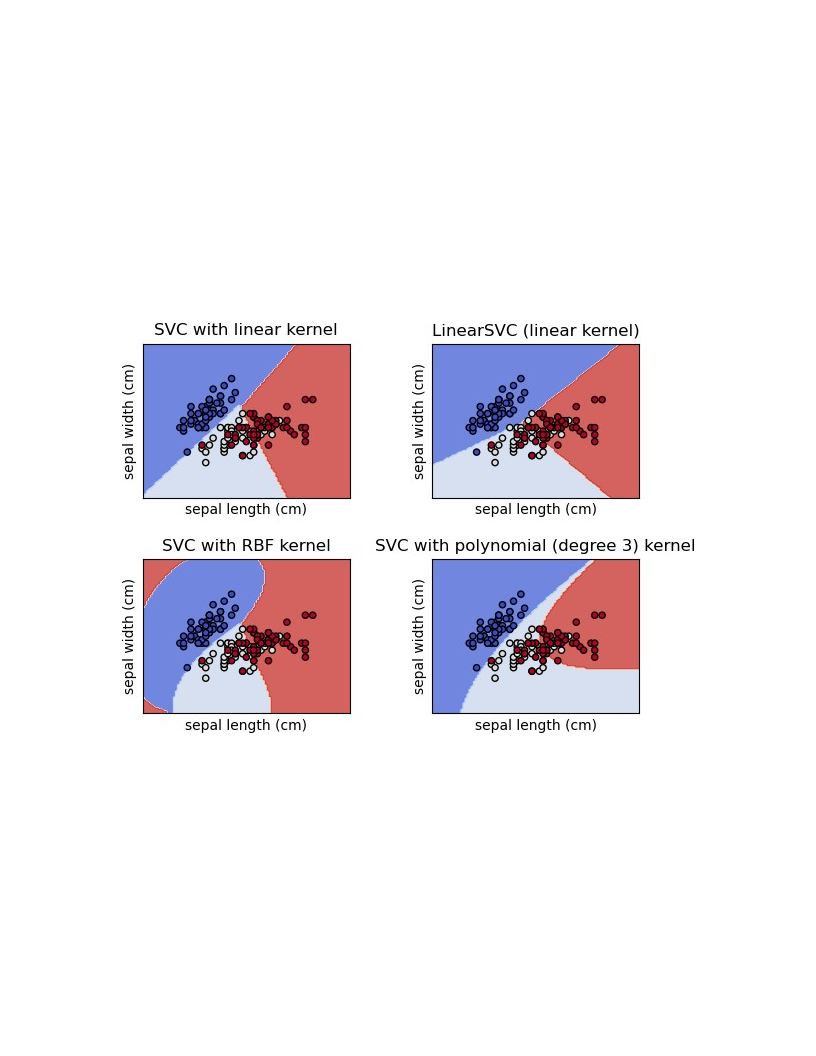
\includegraphics[width=0.6\textwidth]{media/ict/image21}
	\caption*{Figure 5 - Support Vector Machine}
\end{figure}

\begin{multicols}{2}
In the context of thermal comfort prediction, SVM can be utilized to
analyze complex relationships between various environmental factors such
as temperature, humidity, and air velocity, and the corresponding human
thermal comfort responses. By training the SVM model on labeled datasets
containing information about environmental conditions and associated
thermal comfort ratings, the algorithm can learn to predict the level of
thermal comfort for a given set of environmental parameters.

\begin{enumerate}[leftmargin=*]
\def\labelenumi{\Alph{enumi}.}
\setcounter{enumi}{6}
\item
  \emph{Random Forest (RF)}
\end{enumerate}

Random Forest is a popular machine-learning algorithm that can be used
for both classification and regression tasks. It is an ensemble learning
method that combines multiple decision trees to create a more accurate
and stable model.
\end{multicols}

\begin{figure}[H]
	\centering
	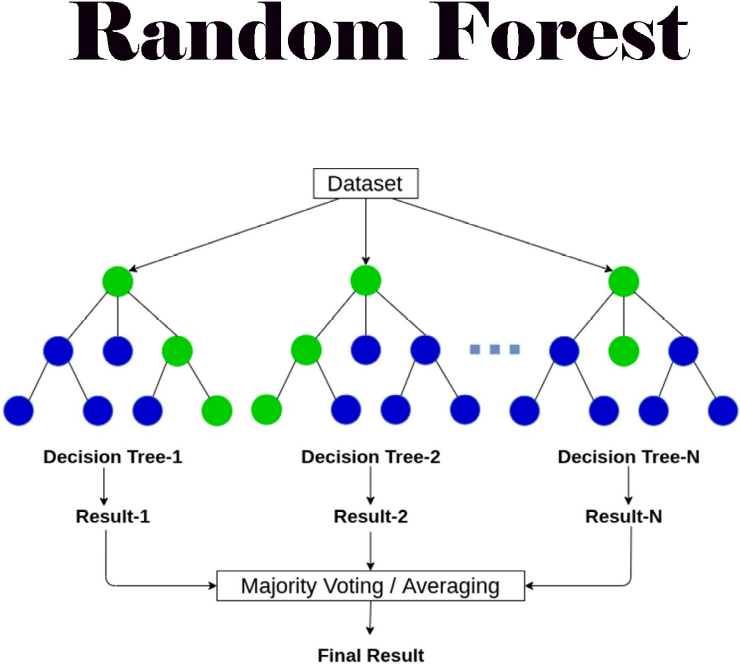
\includegraphics[width=0.5\textwidth]{media/ict/image22}
	\caption*{Figure 6 - Random Forest}
\end{figure}

\begin{multicols}{2}
Data preparation involves cleaning the data, dealing with missing
values, and transforming it to ensure it is suitable for the algorithm.
Random sampling is used to randomly select a subset of the data to use
for training each decision tree. Decision tree creation is created using
recursive partitioning and feature selection. Voting is used to combine
the predictions of all the trees to make the final prediction.
Evaluation is done using a validation set. Overall, the Random Forest
algorithm is a powerful machine-learning method that can be used for a
wide range of tasks. It is easy to use and can produce accurate and
stable predictions even with noisy or incomplete data. When applied to
thermal comfort prediction, Random Forest models excel in capturing
nonlinear relationships and inter- actions among various environmental
factors. By aggregating predictions from multiple decision trees, Random
Forest can provide accurate estimates of thermal comfort levels across
different environmental conditions.

\begin{enumerate}[leftmargin=*]
\def\labelenumi{\Alph{enumi}.}
\setcounter{enumi}{7}
\item
  \emph{Integration with IoT}
\end{enumerate}

The IoT component of the system involves deploying a network of sensors
within the building. These sensors collect real-time data on various
environmental conditions, such as temperature, humidity, CO2 levels, and
occupancy. Data from IoT sensors are transmitted to a central server for
storage and analysis. Wireless communication protocols like Wi-Fi,
Bluetooth, or LoRaWAN can be used for efficient data transfer. The AI
models receive real-time data from the IoT sensors, enabling them to
continuously update predictions and make immediate adjustments to the
HVAC system for optimal ther- mal comfort. An important aspect of the
system is its ability to create a feedback loop that maintains thermal
comfort. The AI algorithms analyze the real-time data from IoT sensors
and make recommendations or control the HVAC system to ensure that
thermal comfort is maintained. For instance, if the system detects a
deviation from the desired comfort level, it can adjust the temperature,
humidity, or airflow accordingly.

\begin{enumerate}[leftmargin=*]
\def\labelenumi{\Alph{enumi}.}
\setcounter{enumi}{8}
\item
  \emph{Alternative prediction value}
\end{enumerate}

So, an alternative way for predicting value we use the Thermal
preference column instead Thermal comfort. If we do not switch from 6
digits to 3 as before.

{\bfseries Results and Discussion.} After filtering, we have 21 columns out
of 70. And we make feature selections using correlation. Moreover, we
avoid choosing Fanger's features. After one more filtering by cor-
relation and with model SelectKbest which will help us to get the list
of features. We get more than 3 variations, but we stopped in those
variants:

\begin{enumerate}[leftmargin=*]
\def\labelenumi{\arabic{enumi})}
\item
  First set of 17 features: (Age, Sex, Met, Thermal pref- erence,
  Thermal sensation, Clo, Subjects height (cm), Subjects weight (kg),
  Year, Season, Koppen climate clas- sification, Building type, Cooling
  strategy building level, Air temperature (C), Outdoor monthly air
  temperature (C), Relative humidity (\%), Air velocity (m/s)).
\item
  Second set of 9 features: (Age, Sex, Met, Clo, Year, Season, Air
  temperature (C), Relative humidity (\%), Air velocity (m/s)).
\item
  Third set of 15 features: (Age, Clo, Sex, Met, Thermal preference,
  Year, Season, Koppen climate classification, Cooling strategy building
  level, City, PPD, Air tempera- ture (C), Outdoor monthly air
  temperature (C), Relative humidity (\%), Air velocity (m/s))
\end{enumerate}

In the end, we have 17 columns and 6765 rows. Starting work, we first
take 17 out of 17 columns, we get not good results. Second iteration we
take 9 out of 17 columns they also give results around the first
iteration. In the last iteration, we take 15 out of 17 columns results
are not good either. For that situation, we tested our hypothesis and
IQR method gives approximately 3-4\% accuracy, and the reducing label
values method gives 20-23\% accuracy. By changing the parameters of the
models we define good parameters for our case then for the SVM model,
the parameters were taken as \emph{kernel} = ''rbf'', \emph{gamma} =
0.001, and \emph{c} = 3. And for the Random Forest, the parameters were
taken as \emph{estimators} = 300, \emph{max depth} = 15. These
parameters gave the maximum accuracy values. The results of comparing
the use of LabelEncoder and OneHotEncoder in the dataset give a 2-4\%
percent difference between them. Regardless of the features, and what
parameters have been entered. This influenced the fact to take
OneHotEncoder. If you do data standardization, the accuracy results will
not change much and remain practically the same. For standardization, we
used StandardScaler and MinMaxScaler models.

Below are presented 1, 2, and 3 tables the beginning results of our
prediction:
\end{multicols}

\begin{table}[H]
\caption*{Table 1 - Iteration of 17 features}
\centering
\begin{tabular}{|l|l|l|l|l|}
\hline
Model & Accuracy & Precision & Recall & F1 				score \\ \hline
SVM   & 0.509    & 0.451     & 0.509  & 0.436        \\ \hline
RF    & 0.543    & 0.505     & 0.543  & 0.5          \\ \hline
\end{tabular}
\end{table}

\begin{table}[H]
\caption*{Table 2 - Iteration of 9 features}
\centering
\begin{tabular}{|l|l|l|l|l|}
\hline
Model & Accuracy & Precision & Recall & F1 				score \\ \hline
SVM   & 0.507    & 0.461     & 0.507  & 0.438        \\ \hline
RF    & 0.526    & 0.513     & 0.526  & 0.49         \\ \hline
\end{tabular}
\end{table}

\begin{table}[H]
\caption*{Table 3 - Iteration of 15 features}
\centering
\begin{tabular}{|l|l|l|l|l|}
\hline
Model & Accuracy & Precision & Recall & F1 				score \\ \hline
SVM   & 0.533    & 0.448     & 0.533  & 0.433        \\ \hline
RF    & 0.54     & 0.475     & 0.539  & 0.482        \\ \hline
\end{tabular}
\end{table}

According above results, we tried to improve accuracy using our
hypothesis. Below presented 4, 5, and 6 tables show the results of
\emph{IQR} method:

\begin{table}[H]
\caption*{Table 4 - Iteration of 17 features with \emph{IQR}}
\centering
\begin{tabular}{|l|l|l|l|l|}
\hline
Model & Accuracy & Precision & Recall & F1 score \\ \hline
SVM   & 0.522    & 0.44      & 0.522  & 0.441    \\ \hline
RF    & 0.548    & 0.517     & 0.548  & 0.504    \\ \hline
\end{tabular}
\end{table}

\begin{table}[H]
\caption*{Table 5 - Iteration of 9 features with \emph{IQR}}
\centering
\begin{tabular}{|l|l|l|l|l|}
\hline
Model & Accuracy & Precision & Recall & F1 score \\ \hline
SVM   & 0.507    & 0.44      & 0.383  & 0.424    \\ \hline
RF    & 0.52     & 0.501     & 0.52   & 0.479    \\ \hline
\end{tabular}
\end{table}

\begin{table}[H]
\caption*{Table 6 - Iteration of 15 features with \emph{IQR}}
\centering
\begin{tabular}{|l|l|l|l|l|}
\hline
Model & Accuracy & Precision & Recall & F1 score \\ \hline
SVM   & 0.563    & 0.539     & 0.563  & 0.425    \\ \hline
RF    & 0.57     & 0.494     & 0.57   & 0.5      \\ \hline
\end{tabular}
\end{table}

From previous results, \emph{IQR} method upgrades accuracy approximately
to 2-5\%. Next, we work with the reduction of label values to increase
the accuracy:

\begin{table}[H]
\caption*{Table 7 - Iteration of 17 features with reducing labels}
\centering
\begin{tabular}{|l|l|l|l|l|}
\hline
Model & Accuracy & Precision & Recall & F1 score \\ \hline
SVM   & 0.715    & 0.644     & 0.715  & 0.614    \\ \hline
RF    & 0.744    & 0.708     & 0.744  & 0.704    \\ \hline
\end{tabular}
\end{table}

\begin{table}[H]
\caption*{Table 8 - Iteration of 9 features with reducing labels}
\centering
\begin{tabular}{|l|l|l|l|l|}
\hline
Model & Accuracy & Precision & Recall & F1 score \\ \hline
SVM   & 0.688    & 0.598     & 0.688  & 0.569    \\ \hline
RF    & 0.699    & 0.657     & 0.699  & 0.645    \\ \hline
\end{tabular}
\end{table}

\begin{table}[H]
\caption*{Table 9 - Iteration of 15 features with reducing labels}
\centering
\begin{tabular}{|l|l|l|l|l|}
\hline
Model & Accuracy & Precision & Recall & F1 score \\ \hline
SVM   & 0.78     & 0.608     & 0.78   & 0.683    \\ \hline
RF    & 0.78     & 0.719     & 0.78   & 0.727    \\ \hline
\end{tabular}
\end{table}

Adding \emph{IQR} method to the reduced features and get such results:


\begin{table}[H]
\caption*{Table 10 - Iteration of 17 features with reducing labels and \emph{IQR}}
\centering
\begin{tabular}{|l|l|l|l|l|}
\hline
Model & Accuracy & Precision & Recall & F1 score \\ \hline
SVM   & 0.726    & 0.598     & 0.726  & 0.621    \\ \hline
RF    & 0.733    & 0.678     & 0.733  & 0.688    \\ \hline
\end{tabular}
\end{table}


\begin{table}[H]
\caption*{Table 11 - Iteration of 9 features with reducing labels and \emph{IQR}}
\centering
\begin{tabular}{|l|l|l|l|l|}
\hline
Model & Accuracy & Precision & Recall & F1 score \\ \hline
SVM   & 0.706    & 0.498     & 0.706  & 0.584    \\ \hline
RF    & 0.717    & 0.668     & 0.717  & 0.653    \\ \hline
\end{tabular}
\end{table}


\begin{table}[H]
\caption*{Table 12 - Iteration of 15 features with reducing labels and
\emph{IQR}}
\centering
\begin{tabular}{|l|l|l|l|l|}
\hline
Model & Accuracy & Precision & Recall & F1 score \\ \hline
SVM   & 0.835    & 0.697     & 0.835  & 0.76     \\ \hline
RF    & 0.821    & 0.738     & 0.821  & 0.766    \\ \hline
\end{tabular}
\end{table}

There was also work on the alternative method. Here Thermal comfort and
Thermal preference will change places. And now we will predict Thermal
preference.

\begin{table}[H]
\caption*{Table 13 - Alternative iteration of 15 features}
\centering
\begin{tabular}{|l|l|l|l|l|}
\hline
Model & Accuracy & Precision & Recall & F1 score \\ \hline
SVM   & 0.68     & 0.714     & 0.68   & 0.605    \\ \hline
RF    & 0.714    & 0.712     & 0.714  & 0.685    \\ \hline
\end{tabular}
\end{table}

\begin{table}[H]
\caption*{Table 14 - Alternative iteration of 15 features with reducing labels}
\centering
\begin{tabular}{|l|l|l|l|l|}
\hline
Model & Accuracy & Precision & Recall & F1 score \\ \hline
SVM   & 0.67     & 0.698     & 0.67   & 0.584    \\ \hline
RF    & 0.705    & 0.702     & 0.705  & 0.673    \\ \hline
\end{tabular}
\end{table}

\begin{table}[H]
\caption*{Table 15 - Alternative iteration of 15 features with reducing labels and \emph{IQR}}
\centering
\begin{tabular}{|l|l|l|l|l|}
\hline
Model & Accuracy & Precision & Recall & F1 score \\ \hline
SVM   & 0.694    & 0.55      & 0.694  & 0.577    \\ \hline
RF    & 0.709    & 0.676     & 0.709  & 0.651    \\ \hline
\end{tabular}
\end{table}

\begin{multicols}{2}
{\bfseries Conclusion.} As a result, we pass a verdict that added
\emph{IQR} method, we worked with new 8 features and 7 features were
already in other articles, considering the option with guessing Thermal
comfort and Thermal preference, the difference between the two
algorithms is 1-3\%. Basically Random Forest looks more stable than SVM.
I would also like to note that the alternative version was in the lead
in 9 and 15 features, Table 3 and Table 13. But, when we started
converting from 6 to 3 Thermal comfort values and added \emph{IQR}
method, our main option immediately won. In the future, I will add new
features to improve accuracy. For example, one of them is Heart Rate
Variability (HRV) {[}11{]}. On top of that, I want to test neural
networks and deep learning as I have seen good results with these
algorithms. I also considered these {[}15, 16{]} papers for the basis of
a new work. Some commonly used algorithms for this purpose include
Convolutional Neural Networks (CNNs), Recurrent Neural Networks (RNNs),
Long Short-Term Memory (LSTM) Networks, Autoencoders, and Deep Belief
Networks (DBNs).
\end{multicols}

\begin{center}
{\bfseries References}
\end{center}

\begin{references}
1. Christos G. Polycarpou, Marios M. Milis, George M. Panayiotou.
Iot-enabled automatic synthesis of distributed feedback control schemes
in smart buildings.// IEEE Internet of Things
Journa\href{https://ieeexplore.ieee.org/xpl/RecentIssue.jsp?punumber=6488907}{l}.-
2021.-Vol.8, Iss.4.- P.2615-2626.
\href{https://doi.org/10.1109/JIOT.2020.3019662}{DOI
10.1109/JIOT.2020.3019662}

2. Mulyana Binti Bin Omar, Ridha Mohamed Salleh and Faridah Hani
Saripuddin. Predicting thermal comfort of hvac building using 6 thermal
factors.//
\href{https://ieeexplore.ieee.org/xpl/conhome/9243083/proceeding}{8th
International Conference on Information Technology and Multimedia
(ICIMU)}.-2020.
\href{https://doi.org/10.1109/ICIMU49871.2020.9243466}{DOI
10.1109/ICIMU49871.2020.9243466}

3. Sara Sorcinelli, Matteo Arnesano, Marco Uriarte, Amaia
Torrens-Galdiz, J. Ignacio Revel, Gian Marco Morresi and Nicole
Casaccia. Sensing physiological and environmental quantities to measure
human thermal comfort through machine learning
techniques//\href{https://ieeexplore.ieee.org/xpl/RecentIssue.jsp?punumber=7361}{IEEE
Sensors Journal}. -2021.-Vol.21. - Iss.10.-P. 12322-12337.
\href{https://doi.org/10.1109/JSEN.2021.3064707}{DOI
10.1109/JSEN.2021.3064707}

4. Juliana Caesarendra, Wahyu Shona Laila, Dina Candra Kurnia, Jundika
Widiastuti and Ratih Zaini. Prediction on the indoor thermal comfort of
occupied room based on iot climate measurement open datasets //
International Conference on Informatics, Multimedia, Cyber and
Information System (ICIMCIS).- 2020.
\href{https://doi.org/10.1109/ICIMCIS51567.2020.9354277}{DOI
10.1109/ICIMCIS51567.2020.9354277}

5. Yadong Xu, Zhanbo Wu, Jiang Liu, Yaping Guo, Yuntao Guan, Xiaohong Su
and Ying Zhou. Group comfort models: Predicting indoor group thermal
comfort by learning preferences of multiple occupants.//
IEEE 16th International Conference on Automation Science and Engineering
(CASE).- 2020. DOI

\href{https://doi.org/10.1109/CASE48305.2020.9216834}{10.1109/CASE48305.2020.9216834}

6. M. Hani Mohamed Salleh and Faridah Binti Saripuddin. Monitoring
thermal comfort level of commercial buildings' occupants in a hot-humid
climate country using k-nearest neighbors model.//
\href{https://ieeexplore.ieee.org/xpl/conhome/9233041/proceeding}{5th
International Conference on Power and Renewable Energy (ICPRE)}.- 2020.
DOI 10.1109/ICPRE51194.2020.9233145

7. Moez Merghem-Boulahia, Leila Khalil and Maysaa Esseghir. An iot
environment for estimating occupants' thermal comfort//
\href{https://ieeexplore.ieee.org/xpl/conhome/9210501/proceeding}{IEEE
31st Annual International Symposium on Personal, Indoor and Mobile Radio
Communications}.- 2020. https://doi.org/10.1109/PIMRC48278.2020.9217157

8. Manisa Chen, Tao Rahman, Saifur Zhang and Xiangyu Pipattanasomporn.
An iot-based thermal model learning framework for smart buildings.//
\href{https://ieeexplore.ieee.org/xpl/RecentIssue.jsp?punumber=6488907}{IEEE
Internet of Things Journal}.-~Vol.
7,~\href{https://ieeexplore.ieee.org/xpl/tocresult.jsp?isnumber=8955685&punumber=6488907}{Iss.
1}.-2020.-P. 518-52.
\href{https://doi.org/10.1109/JIOT.2019.2951106}{DOI
10.1109/JIOT.2019.2951106}

9. Asif Irshad Irfan, Sayed Ameenuddin Alam, Md Mottahir Almalawi,
Abdulmohsen Zahir, Md Hasan Irshad and Kashif Khan. Utilizing artificial
neural network for prediction of occupants thermal comfort: A case study
of a test room fitted with a thermoelectric air-conditioning system.//
\href{https://ieeexplore.ieee.org/xpl/RecentIssue.jsp?punumber=6287639}{IEEE
Access}.-Vol. 8-2020.-P. 99709~-- 99728. DOI 10.1109/ACCESS.2020.2985036

10. Jie Wen, Yonggang Gao and Guanyu Li.Deepcomfort: Energy-efficient
thermal comfort control in buildings via reinforcement learning.// IEEE
Internet of Things Journal. -- 2020. - Vol. 7(9). --P. 8472-8484 DOI
10.1109/JIOT.2020.2992117

11. Burak Shi, Zixiao Shen, Weiming Yang and Chunsheng Gunay. Machine
learning-based prognostics for central heating and cooling plant
equipment health monitoring.// IEEE Transactions on Automation Science
and Engineering/. -- 2021.- Vol.18(1).- P.~346--355. DOI
10.1109/TASE.2020.2998586

12. Hiroshi Matsuhashi, Ryuji Wang and Ziyang Onodera,. Proposal of
relative thermal sensation: Another dimension of thermal comfort and its
investigation.// IEEE Access. -- 2021.- P.(99):1-1 

DOI 10.1109/ACCESS.2021.3062393

13. Yonggang Tseng, King Jet Jin, Guangyu Zhang and Wei Wen.
Demystifying thermal comfort in smart buildings: An interpretable
machine learning approach.//
\href{https://ieeexplore.ieee.org/xpl/RecentIssue.jsp?punumber=6488907}{IEEE
Internet of Things Journal}.-2021.-Vol.8,Iss.10.-P.8021-8031.
\href{https://doi.org/10.1109/JIOT.2020.3042783}{DOI
10.1109/JIOT.2020.3042783}

14. SHRAE dataset, ``ASHRAE Global Thermal Comfort Database II'\,',
2020, \href{https://www.kaggle.com/datasets/claytonmiller/ashrae-global-thermal-comfort-database-ii}{https://www.kaggle.com}

15. Nivethitha Somu, Anirudh Sriram, Anupama Kowli, Krithi Ramamritham.
A hybrid deep transfer learning strategy for thermal comfort prediction
in
buildings//\href{https://www.sciencedirect.com/journal/building-and-environment}{Building
and Environment}.-2021.- Vol.204: 108133.
\href{https://doi.org/10.1016/j.buildenv.2021.108133}{DOI
10.1016/j.buildenv.2021.108133}

16. Hansaem Park, Dong Yoon Park Prediction of individual thermal
comfort based on ensemble transfer learning method using wearable and
environmental sensors//
\href{https://www.sciencedirect.com/journal/building-and-environment}{Building
and Environment}.-2022.- Vol.207: 108492. DOI
10.1016/j.buildenv.2021.108492
\end{references}

\begin{authorinfo}
\hspace{1em}\emph{{\bfseries Information about the authors}}

Assymkhan N.B. -- master of Kazakh-British Technical University, e-mail:
\href{mailto:anb.asymhan@gmail.com}{\nolinkurl{anb.asymhan@gmail.com}};

Kartbaev A.Z. -- PhD, Associate professor, Kazakh-British Technical University, e-mail:
a.kartbaev@kbtu.kz;

\hspace{1em}\emph{{\bfseries Сведения об авторах}}

Асымхан Н.Б. -- магистрант Казахстанско-Британский Технического
Университета, e-mail:
\href{mailto:anb.asymhan@gmail.com}{\nolinkurl{anb.asymhan@gmail.com}};

Картбаев А. -- PhD, ассоциированный профессор, Казахстанско-Британский Технического Университета,
e-mail:
\\\href{mailto:a.kartbaev@kbtu.kz}{\nolinkurl{a.kartbaev@kbtu.kz}};
\end{authorinfo}
